During the development of the application, various design patterns were incorporated to efficiently address specific challenges. Different sectors of the application required distinct patterns, particularly in the interactive editor and tool functionalities. Given the complexity of these components, tailored solutions were necessary. For instance, implementing an undo functionality—a widely expected usability feature in modern editors, both text-based and visual—required careful design considerations. This feature is commonly applied across software products, with multiple solutions available. Specialized implementations of design patterns were employed in the following aspects of the application:
\begin{compactitem}
\item Undo/Redo functionality of Actions
\item Tool System
\item Backend services
\end{compactitem}

\subsection{Undo/Redo}
\label{sec:undo-redo}

The undo/redo mechanism is essential for usability, providing users with the flexibility to revert and reapply actions efficiently. Multiple approaches exist for implementing this feature:

\begin{compactenum}
\item \textbf{State Snapshot Approach}: This method involves saving the entire application state at each change and reverting to the previous state when undoing. While simple to implement, this approach is inefficient due to excessive memory consumption and redundant data storage. An advantage is that old states can easily be restored without any additional logic and calculations. This makes it less prone to bugs and errors.
\item \textbf{Differential State Storage}: Instead of storing complete states, this approach records only the differences between successive states, similar to version control systems such as Git. While more efficient, this method becomes complex as the number and types of objects increase (in this case it would be Seats and Standing-Areas).
\item \textbf{Command Pattern}: Actions are encapsulated as objects that implement a common interface, containing methods for execution and reversal. This approach allows flexible and scalable undo/redo functionality, making it ideal for complex interactive applications. It also allows executing additional business logic when undoing an action, like deleting additional data that was created by the action, or sending requests to a backend. This makes it an excellent choice when states are distributed.
\item \textbf{Memento Pattern}: This pattern captures and externalizes an object's internal state so that it can be restored later without violating encapsulation. While useful for preserving an object's complete state, it can be memory-intensive when storing multiple versions.
\end{compactenum}

Given the application's complexity, a variation of the Command Pattern has been implemented for the undo/redo functionality. This approach ensures scalability, efficiency, and maintainability while minimizing redundancy of data and code.


\begin{figure}
    \centering
    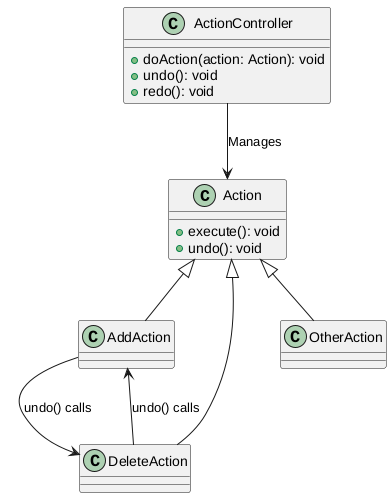
\includegraphics[scale=0.5]{pics/command-pattern.png}
    \caption{Command Pattern in SeatGen}
    \label{fig:command-pattern}
\end{figure}

The implementation defines an abstract \texttt{Action} class that all actions must implement. An overview of this is seen in \ref{fig:command-pattern}. This class enforces the inclusion of \texttt{execute} and \texttt{undo} methods, ensuring a standardized approach to action management.

\begin{lstlisting}[language=TypeScript,caption={Action class},label={lst:action-class}]
export abstract class Action {
    execute: (() => void) | undefined;
    undo: (() => void) | undefined;
}
\end{lstlisting}

For both of these properties a function is expected that can be called to execute the action or to undo the \texttt{Action}. This is a flexible approach and can be used for a lot of different actions. 

Another important aspect of this application was to allow the execution of business logic while undoing specific actions, like sending requests to the backend. This is very easy to implement because each Action has its individual \texttt{execute} and \texttt{undo} function.

While this seems like a lot more logic is needed than in the other design patterns, the logic demanded by this is actually important for usability reasons, and lots of it is reusable. Because the undo function should be able to be executed manually by the user, calling the \texttt{undo()} shouldn't be the only way to reverse an action, for example when creating a new seat, you should be able to delete it again by calling the \texttt{undo()} function as well as a separate way like a delete button. So the developer should always provide both ways for usability reasons. This approach incentivizes developers to do it because it's mandatory to implement the logic for undoing an action anyway.

Here is an implementation of an action that creates a Standing-Area with its counterpart action that deletes the standing area. Both actions can reference each other for the undoing part to reduce code redundancy, because the opposite of creating a standing area is deleting it. That's why deleting it is the undo action of creating it and the other way around.

\begin{lstlisting}[language=TypeScript,caption={Add standing-area action implementation},label={lst:add-standing-area-action-implementation}]
export class AddStandingAreaAction implements Action {
    private readonly _newArea: StandingArea;
    private readonly _context: MapContextValue;

    constructor(newArea: StandingArea, context: MapContextValue) {
        this._newArea = newArea;
        this._context = context;
    }

    execute = () => {
        this._context.setStandingAreas((prevAreas) => 
            [...prevAreas, this._newArea]
        );
        if (this._context.standingAreasToDelete.includes(this._newArea.id))
        {
            this._context.setStandingAreasToDelete((prev) =>
                prev.filter(id => id !== this._newArea.id)
            );
        } else {
            this._context.setStandingAreasToSave((prev) => {
                const updated = [...prev, this._newArea.id];
                return updated;
            });
        }
    };

    undo = () => {
        new DeleteStandingAreaAction([this._newArea], this._context).execute()
    };
}
\end{lstlisting}

\begin{lstlisting}[language=TypeScript,caption={Delete standing-area action implementation},label={lst:delete-standing-area-action-implementation}]
export class DeleteStandingAreaAction implements Action {
    private readonly _deletedAreas: StandingArea[];
    private _undoAreas: StandingArea[] | undefined;
    private readonly _context: MapContextValue;

    constructor(deletedAreas: StandingArea[], context: MapContextValue) {
        this._deletedAreas = deletedAreas;
        this._context = context;
    }

    execute = () => {
        const deletedAreaIds = this._deletedAreas.map(area => area.id);
        this._context.setStandingAreas((prevAreas) =>
            prevAreas.filter((area) => !deletedAreaIds.includes(area.id))
        );
        this._context.setStandingAreasToDelete((prev) => 
            [...prev, ...deletedAreaIds]
        );
        deletedAreaIds.forEach(id => {
            if (this._context.standingAreasToSave.includes(id)) 
            {
                this._context.setStandingAreasToSave(this._context
                .standingAreasToSave
                .filter(savedId => savedId !== id));
            } else 
            {
                this._context.setStandingAreasToDelete((prev) => [...prev, id]);
            }
        });
    }

    undo = () => {
        if (this._undoAreas) {
            this._deletedAreas.forEach((area) => {
                new AddStandingAreaAction(area, this._context).execute()
            })
        }
    }
}
\end{lstlisting}

In the code in Listing \ref{lst:add-standing-area-action-implementation} and \ref{lst:delete-standing-area-action-implementation} you have the functions with the business logic for creating and deleting a standing area. When the \texttt{undo()} function is called, actually a new \texttt{DeleteStandingAreaAction} is created, and its \texttt{execute()} function is called, because it implements the correct business logic for undoing the action. Same is true for the call of the \texttt{undo()} function in the \texttt{DeleteStandingAreaAction}. With this code both functionalities can be implemented by separate buttons or other components, and the undo and redo functionality is implemented as well. The needed contexts and functions to execute the business logic correctly for both classes can be defined individually in the constructor of the classes. The class also has to store the information to undo its actions, for example the move action has to store the old position of the object to be able to move it back to the old position.

The actual undoing logic is defined by a controller. When an action should be undoable and redoable it has to be passed to the controller. The controller manages the function and can be called to undo or redo the last action. It also manages the stack of actions, so that all the actions can be undone and then redone again, until a new action is executed. When this happens the controller ignores all the ``future'' actions that would have come after the current action. For example: Action1, Action2, Action3 and Action4 have been executed. The latest action saved by the controller is currently Action4. Currently, all the actions can be undone and then redone in a stack-like way. This means Action4 is undone, then Action3, then Action2 and so on. Then they can all be reapplied in the same reversed order. When actions have been undone, to Action2 for example, and then a new Action5 is executed, Action3 and Action4 will be scrapped, because a new ``future'' has been created. This is a common behavior in undo and redo functionalities.

The implementation of the controller is as shown in listing \ref{lst:action-controller}.

\begin{lstlisting}[language=TypeScript,caption={Action controller implementation},label={lst:action-controller}]
const loopSize = 50;
const actionHistory: (Action | undefined)[] = new Array(loopSize).fill(undefined);

let historyIndex = 0;
let maxIndex = 0;
let minIndex = -1;
let savedIndex = 0


const doAction = (action: Action) => {
    historyIndex = increase(historyIndex);

    while (maxIndex != historyIndex) {
        actionHistory[maxIndex] = undefined
        maxIndex = decrease(maxIndex)
    }

    actionHistory[minIndex] = undefined
    minIndex = increase(maxIndex);
    actionHistory[historyIndex] = action;
    action.execute!();
    checkForUnsavedChanges()
};

const updateSaveIndex = () => {
    savedIndex = historyIndex
    checkForUnsavedChanges()
}

function increase(num: number): number {
    return num !== loopSize - 1 ? num + 1 : 0;
}

function decrease(num: number): number {
    return num !== 0 ? num - 1 : loopSize - 1;
}

const undo = () => {
    if (historyIndex !== minIndex && actionHistory[historyIndex] !== undefined) {
        actionHistory[historyIndex]!.undo!()
        historyIndex = decrease(historyIndex);
        checkForUnsavedChanges()
        enqueueSnackbar("Undone", {variant: "info"})
    }
};

const redo = () => {
    if (historyIndex !== maxIndex && actionHistory[increase(historyIndex)] !== undefined) {
        historyIndex = increase(historyIndex);
        actionHistory[historyIndex]!.execute!();
        checkForUnsavedChanges()
    }
};

const getCurrentAction = (): Action | null => actionHistory[historyIndex] ?? null;
\end{lstlisting}

To register a new Action in the controller, the \texttt{doAction} function has to be called with the action as a parameter like in this Listing \ref{lst:register-action}. The context referenced here contains the business logic for the map as well as the logic for the undo and redo controller.

\begin{lstlisting}[language=TypeScript,caption={Registering a new action in the controller},label={lst:register-action}]
context.doAction(new AddSeatAction(context.setSeats, lat, lng))
\end{lstlisting}

This controller stores all the actions in the form of a loop, with the size defined by the \texttt{loopSize} variable. The variable is set to 50 because more than 50 undoable actions back are not necessary. A circular buffer for storing this kind of data is very advantageous because when the buffer is full, the oldest action is overwritten by the newest action because the oldest data is not needed anymore. Other very important variables are the \texttt{minIndex} and \texttt{maxIndex} variables. They define the range of the actions that can be undone and redone. When undoing, it's checked that the current index which is represented by the \texttt{historyIndex} is not the same as the \texttt{minIndex} and there is also an undoable action, because then there would be no more actions to undo. Only if these conditions are fulfilled, there are actions to undo, and the \texttt{undo()} function can be called and the \texttt{historyIndex} can be decreased. A similar logic is applied for the \texttt{redo()} function, but with the \texttt{maxIndex} and the \texttt{increase()} function. The \texttt{doAction()} function is used to handle new actions. It increases the \texttt{historyIndex} and sets the \texttt{maxIndex} to the \texttt{historyIndex} and overwrites all the no longer needed actions with undefined. The \texttt{minIndex} is set to the \texttt{increase(maxIndex)} to ensure that when the loop is full, changes that are too old get removed. At last the action is added to the list of actions and the \texttt{execute()} function is called.

The \texttt{increase()} and \texttt{decrease()} functions are used to increase and decrease the index in a circular way. This is necessary because the buffer is circular and when the end of the buffer is reached, the index has to be set to the beginning of the buffer again. This is done by checking if the index is at the end of the buffer and then setting it to the beginning of the buffer again.

\subsection{Tools}
Tools played a significant role during development, making it essential to ensure that the implementation of new tools was as easy and fast as possible. To achieve this, a Tool interface was designed, where instances only need to be added to an existing array containing the tools. The final version of this interface is presented in Listing. \ref{lst:tool-interface}.

\begin{lstlisting}[language=TypeScript,caption={Tool interface},label={lst:tool-interface}]
export interface Tool {
    id: string
    icon: ReactNode,
    onSelect?: ()=>void,
    hotkey?: string
}
\end{lstlisting}

The attributes of the interface are the following:
\begin{compactitem}
\item \textbf{id}: The id is a string with the name of the tool.
\item \textbf{icon}: The icon of the tool, which is displayed in the toolbar. This has the type \texttt{ReactNode} because first a simple string was used to pass it to an icon component, but then it was decided to use the \texttt{ReactNode} type, because it's more flexible and the icons are not only limited to the icons of one UI library, but any icon can be used, including SVG icons.
\item \textbf{onSelect}: The function that is called when the tool is selected. This is optional because not every tool needs a function to be called when it's selected. Some tools are handled externally.
\item \textbf{hotkey}: The hotkey is a string that defines the hotkey for the tool. This is optional because not every tool needs a hotkey.
\end{compactitem}

Listing \ref{lst:implemented-tools} shows all the implemented tools, and Figure \ref{fig:tools} illustrates how they are rendered.

\begin{lstlisting}[language=TypeScript,caption={Implemented Tools},label={lst:implemented-tools}]
const tools: Tool[] = [
    {
        id: "mouseTool",
        icon: <svg viewBox="0 0 24 24" xmlns="http://www.w3.org/2000/svg">
            <path
                d="..."
            />
        </svg>,
        onSelect: () => handleToolSelect(() => {
        }, "mouseTool", "default"),
        hotkey: "v"
    },
    {
        id: "addTool",
        icon: <PlusIcon></PlusIcon>,
        onSelect: () => handleToolSelect((e) => {
            props.addSeat(e.latlng.lat, e.latlng.lng)
        }, "addTool", "cell"),
        hotkey: "c"
    },
    {
        id: "addGridTool",
        icon: <TableCellsIcon></TableCellsIcon>,
        onSelect: () => handleToolSelect(() => {
        }, "addGridTool", "cell"),
        hotkey: "g"
    },
    {
        id: "squareSelectTool",
        icon: <svg xmlns="http://www.w3.org/2000/svg" viewBox="0 -960 960 960">
            <path
                d="..."/>
        </svg>,
        onSelect: () => handleToolSelect(() => console.log("Clicked"), "squareSelectTool", "crosshair"),
        hotkey: "a"
    },
    {
        id: "standingAreaTool",
        icon: <UserGroupIcon />,
        onSelect: () => handleToolSelect(() =>console.log("standingtool"), "standingAreaTool", "crosshair"),
        hotkey: "s"
    }
];
\end{lstlisting}

\begin{figure}
    \centering
    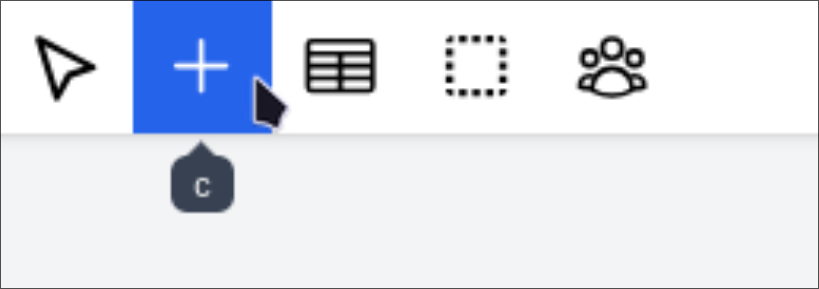
\includegraphics[scale=0.2]{pics/toolbar.png}
    \caption{Tools in SeatGen}
    \label{fig:tools}
\end{figure}


The \texttt{handleToolSelect} function is a function that is called when a tool is selected. It's responsible for setting the current tool and the cursor as shown in listing \ref{lst:handle-tool-select}. All the cursor icons supported by the browser can be utilized by passing their respective names to the function. The cursor names can be viewed on the Mozilla developer documentation \cite{MDNCursor}.

\begin{lstlisting}[language=TypeScript,caption={Handle tool select function},label={lst:handle-tool-select}]
const handleToolSelect = useCallback((toolFunction: (e: LeafletMouseEvent) => void, toolId: string, cursorIcon?: string) => {
    const cursorName = L.DomUtil.getClass(props.map.current!.getContainer()).split(" ").find((it) => it.startsWith("cursor-"));
    if (cursorName) {
        L.DomUtil.removeClass(props.map.current!.getContainer(), cursorName);
    }
    if (cursorIcon !== undefined) {
        L.DomUtil.addClass(props.map.current!.getContainer(), `cursor-${cursorIcon}`);
    }
    setActiveToolFunction(() => toolFunction);
    context.setSelectedToolId(toolId);
}, [props.map, setActiveToolFunction]);
\end{lstlisting}

After all this is set, the tools are simply rendered with a component that handles properties such as hotkeys and the icon.

\subsection{Backend Services}
For the backend services SeatGen uses a very general and exchangeable approach that works with Spring. For the services, an interface is defined, which is then implemented by the respective service classes. This interface is used to define the methods that are needed for the services. In the controller the service is injected, and spring automatically creates an instance of the correct service implementation and injects it into the controller. This is a very common approach in Spring and is used in many projects.